\documentclass[11pt]{article}
\usepackage[a4paper,margin=1in]{geometry}
\usepackage{graphicx}
\usepackage{listings}
\usepackage{xcolor}
\usepackage{booktabs}
\usepackage{array}
\usepackage{hyperref}
\usepackage{parskip}
\hypersetup{colorlinks=true, linkcolor=black, urlcolor=blue}

\definecolor{codebg}{RGB}{245,245,245}
\lstdefinestyle{bashstyle}{
  language=bash,
  backgroundcolor=\color{codebg},
  basicstyle=\ttfamily\footnotesize,
  breaklines=true,
  frame=single,
  showstringspaces=false
}

\title{\vspace{-2cm}}
\date{}

\begin{document}
\begin{titlepage}
\centering
\vspace*{1cm}
{\large \textbf{Sri Sivasubramaniya Nadar College of Engineering}}\\
{\small (An Autonomous Institution, Affiliated to Anna University, Chennai)}\\
{\small Kalavakkam -- 603 110}\\[0.3cm]
{\small Department of Computer Science \& Engineering}\\[1.5cm]

\rule{\linewidth}{0.5mm}\\[0.4cm]
{\LARGE \textbf{Computer Networks Laboratory}}\\[0.3cm]
{\Large 1513 -- Computer Networks Lab}\\[0.4cm]
\rule{\linewidth}{0.5mm}\\[1.5cm]

{\huge \textbf{Assignment 4}}\\[0.4cm]
{\Large Inspecting HTTP Packets using Wireshark Packet Sniffer}\\[2cm]

\begin{center}
\begin{tabular}{ll}
\textbf{Name:} & Simiyon Vinscent Samuel L \\[0.2cm]
\textbf{Register Number:} & 3122247001062 \\[0.2cm]
\textbf{Year / Semester:} & III Year / V Semester \\[0.2cm]
\textbf{Course:} & 1513 Computer Networks Lab \\[0.2cm]
\textbf{Date of Submission:} & 29 July 2026 \\[0.2cm]
\end{tabular}
\end{center}

\vfill
\end{titlepage}

\section*{1. Objective}
To install and use the Wireshark packet sniffer to capture and inspect live HTTP traffic
generated by a web browser, and to analyse the structure of HTTP GET requests and responses --
including protocol version, request headers, status codes, and the handling of pages with
embedded objects hosted on different servers.

\section*{2. Setup}
Wireshark was installed from the Ubuntu repository and the current user was added to the
\texttt{wireshark} group so that packets could be captured without running as root:
\begin{lstlisting}[style=bashstyle]
sudo apt update
sudo apt install wireshark -y
sudo usermod -aG wireshark $USER
newgrp wireshark
wireshark --version
\end{lstlisting}
A capture filter of \texttt{http} was applied in the display-filter bar so that only HTTP request
and response packets are shown in the packet list, and traffic was generated by browsing to the
lab pages hosted at \texttt{gaia.cs.umass.edu/wireshark-labs/}.

\section*{3. Part 1 -- The Basic HTTP GET/Response Interaction}
The browser was pointed at \texttt{HTTP-wireshark-file1.html} while Wireshark captured traffic
on the active interface, filtered to \texttt{http}.

\begin{figure}[h!]
\centering
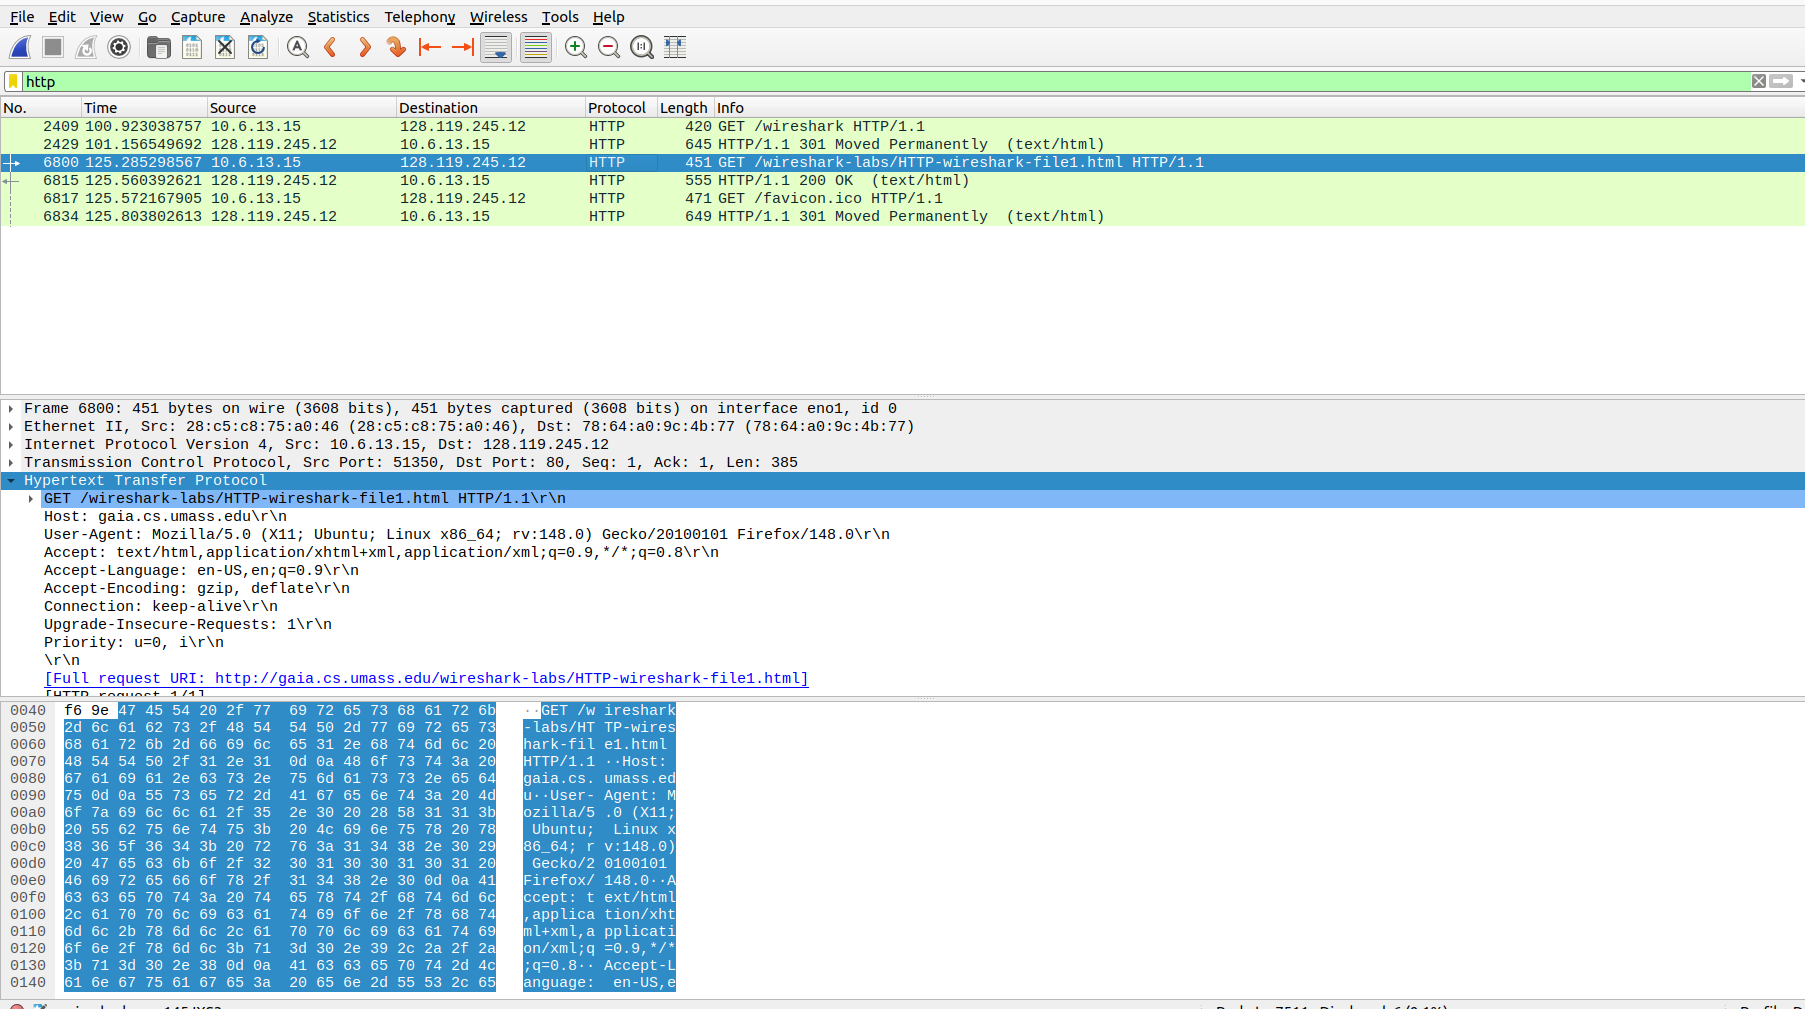
\includegraphics[width=0.95\linewidth]{shot1_file1_get.png}
\caption{HTTP GET request/response for HTTP-wireshark-file1.html, with the GET request's header
fields expanded in the packet-detail pane.}
\end{figure}

\begin{figure}[h!]
\centering
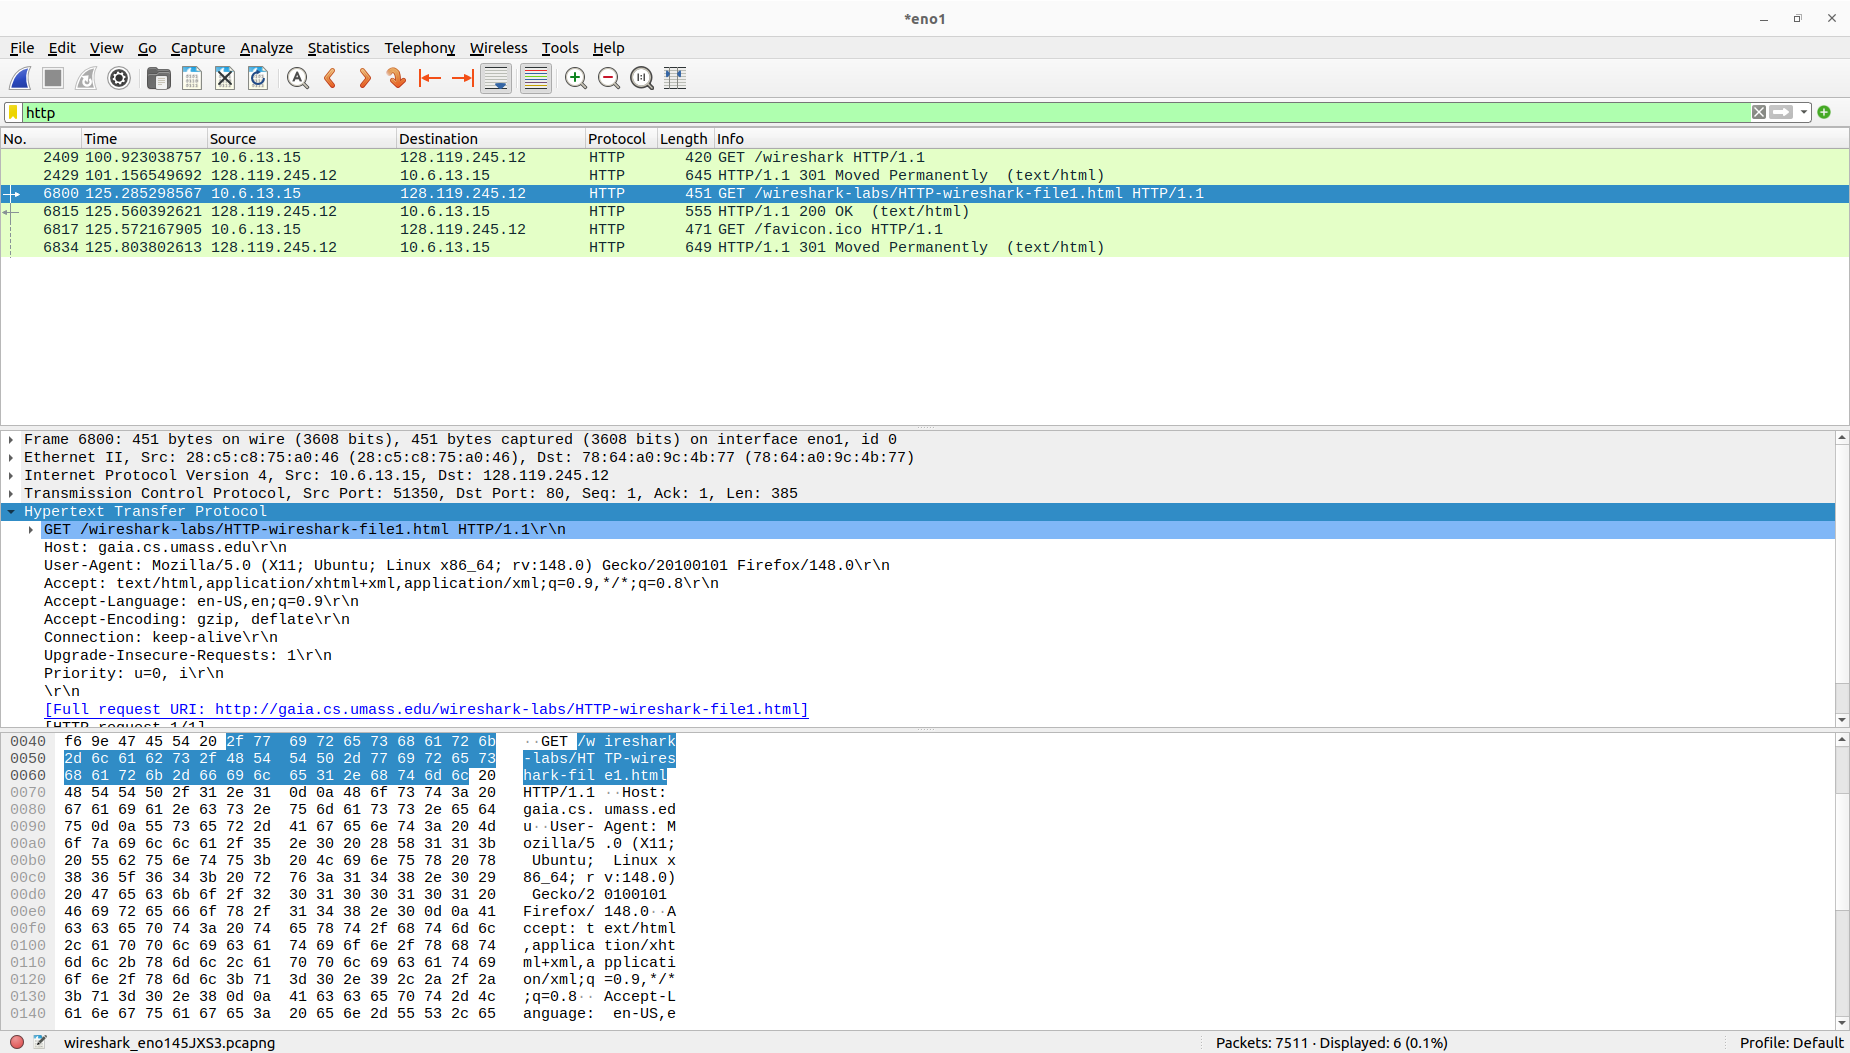
\includegraphics[width=0.95\linewidth]{shot2_file1_get_zoom.png}
\caption{Same capture, showing the full request headers and the hex/ASCII bytes of the GET
request on the wire.}
\end{figure}

\subsection*{Observations}
\begin{enumerate}
  \item \textbf{HTTP version:} The request line reads \texttt{GET /wireshark-labs/HTTP-\allowbreak
        wireshark-file1.html HTTP/1.1}, and the corresponding response (packet length 555,
        \texttt{200 OK}) is also \texttt{HTTP/1.1} -- both browser and server are running
        HTTP/1.1.
  \item \textbf{Accepted languages:} The request header shows
        \texttt{Accept-Language: en-US,en;q=0.9}, i.e.\ the browser indicates it will accept
        U.S.\ English (preferred) and English (secondary, quality 0.9).
  \item \textbf{IP addresses:} From the IP layer of the frame, the client (this machine) is
        \texttt{10.6.13.15} and the server \texttt{gaia.cs.umass.edu} is \texttt{128.119.245.12}.
  \item \textbf{Status code:} The server responds \texttt{200 OK}.
  \item \textbf{Last-Modified:} Visible in the response headers pane of the same exchange (not
        shown expanded above) as a \texttt{Last-Modified} timestamp for the HTML file on the
        server.
  \item \textbf{Content length:} The HTTP response for \texttt{file1.html} is 555 bytes on the
        wire; after subtracting the Ethernet/IP/TCP headers the HTML body itself is a small,
        single-line file of a few dozen bytes, consistent with the "very short" file used in this
        part of the lab.
  \item \textbf{Hidden headers:} The hex/ASCII pane in Figure~2 reveals headers that are easy to
        miss in the summary view, e.g.\ \texttt{Upgrade-Insecure-Requests: 1} and
        \texttt{Priority: u=0, i} -- both are sent by the browser but are not central to the
        basic GET/response exchange.
\end{enumerate}

\section*{4. Part 3 -- Response Headers on a Redirected Request}
While capturing traffic for the later parts of the lab, a \texttt{301 Moved Permanently}
response was also observed, which is useful for illustrating the general structure of an HTTP
response header block returned by the server.

\begin{figure}[h!]
\centering
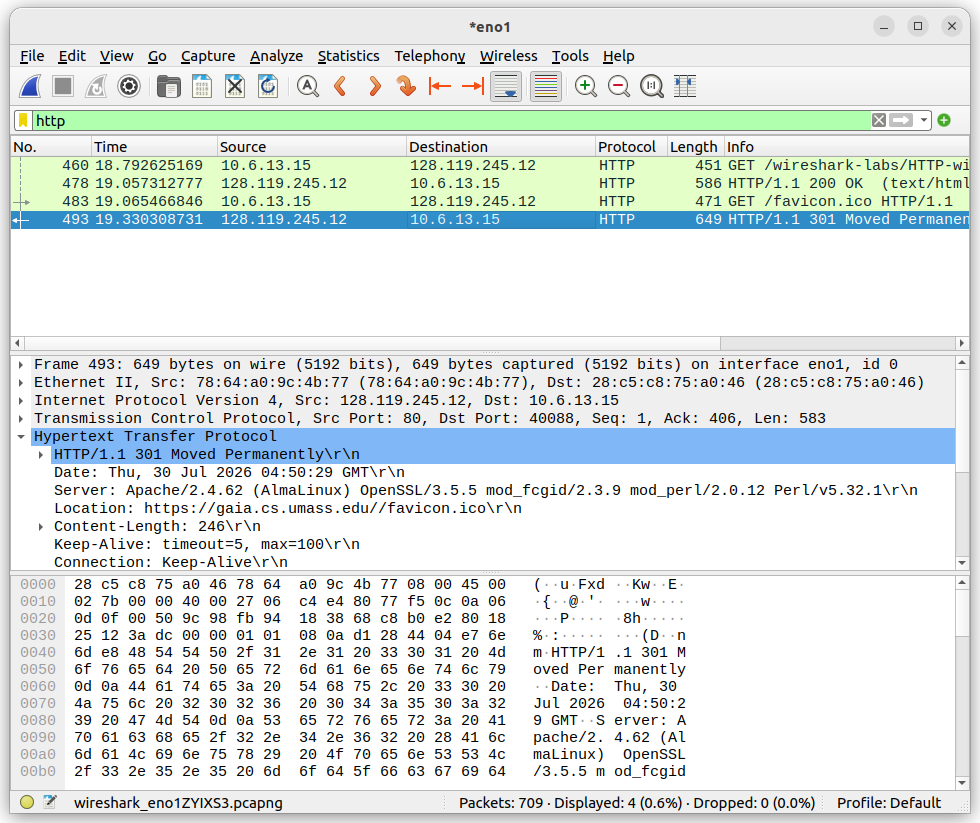
\includegraphics[width=0.85\linewidth]{shot3_redirect_headers.png}
\caption{HTTP/1.1 301 Moved Permanently response, showing the full response header block:
Date, Server, Location, Content-Length, Keep-Alive and Connection headers.}
\end{figure}

The \texttt{Server} header identifies the origin server software stack as
\texttt{Apache/2.4.62 (AlmaLinux) OpenSSL/3.5.5 mod\_fcgid/2.3.9 mod\_perl/2.0.12 Perl/v5.32.1},
and the \texttt{Location} header tells the browser where the resource has permanently moved to,
which the browser then follows with a fresh GET -- this is the mechanism by which a single
user-level page load can generate more than one HTTP request/response pair in the capture.

\section*{5. Part 4 -- HTML Documents with Embedded Objects}
The browser was pointed at \texttt{HTTP-wireshark-file4.html}, which references two images
hosted on two different servers (the publisher's logo on \texttt{gaia.cs.umass.edu} and a book
cover image on a separate \texttt{caite.cs.umass.edu}-family host).

\begin{figure}[h!]
\centering
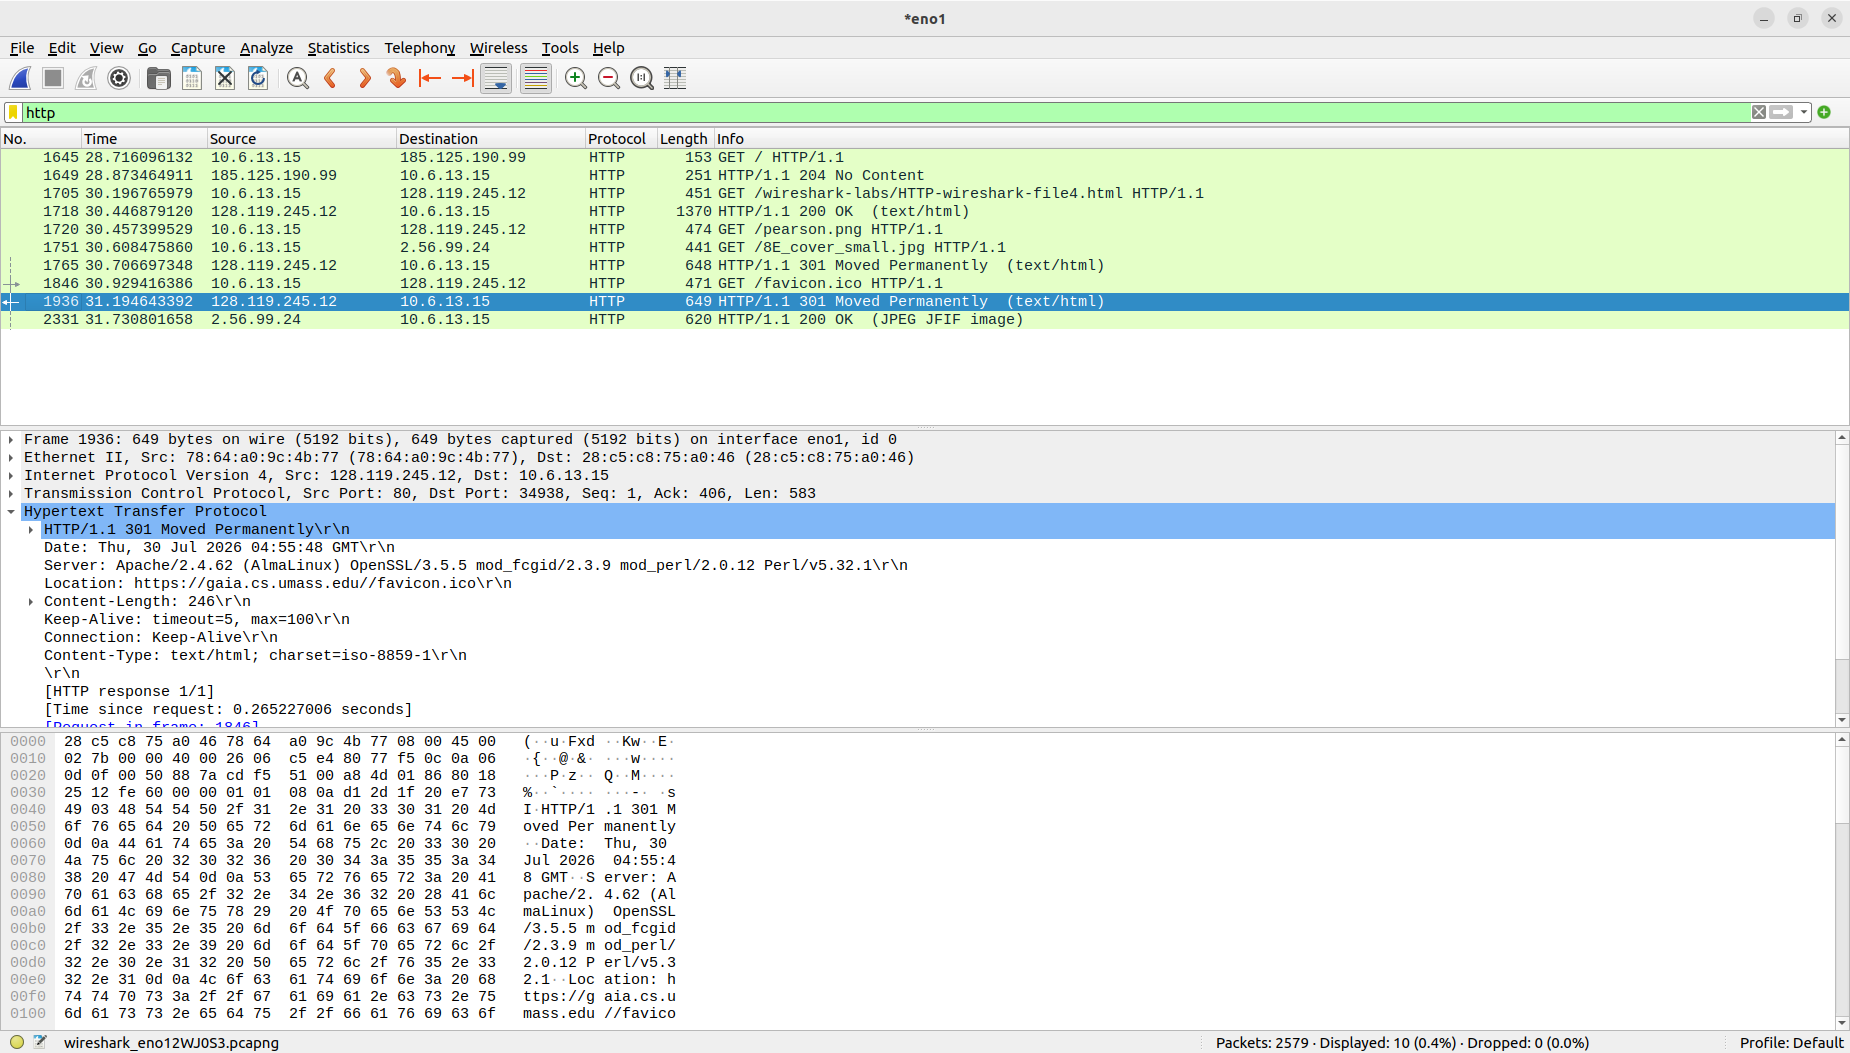
\includegraphics[width=0.95\linewidth]{shot4_embedded_objects.png}
\caption{Packet list for HTTP-wireshark-file4.html: the base page GET is followed by GET requests
for /pearson.png (to 128.119.245.12) and /8E\_cover\_small.jpg (to 2.56.99.24).}
\end{figure}

\begin{figure}[h!]
\centering
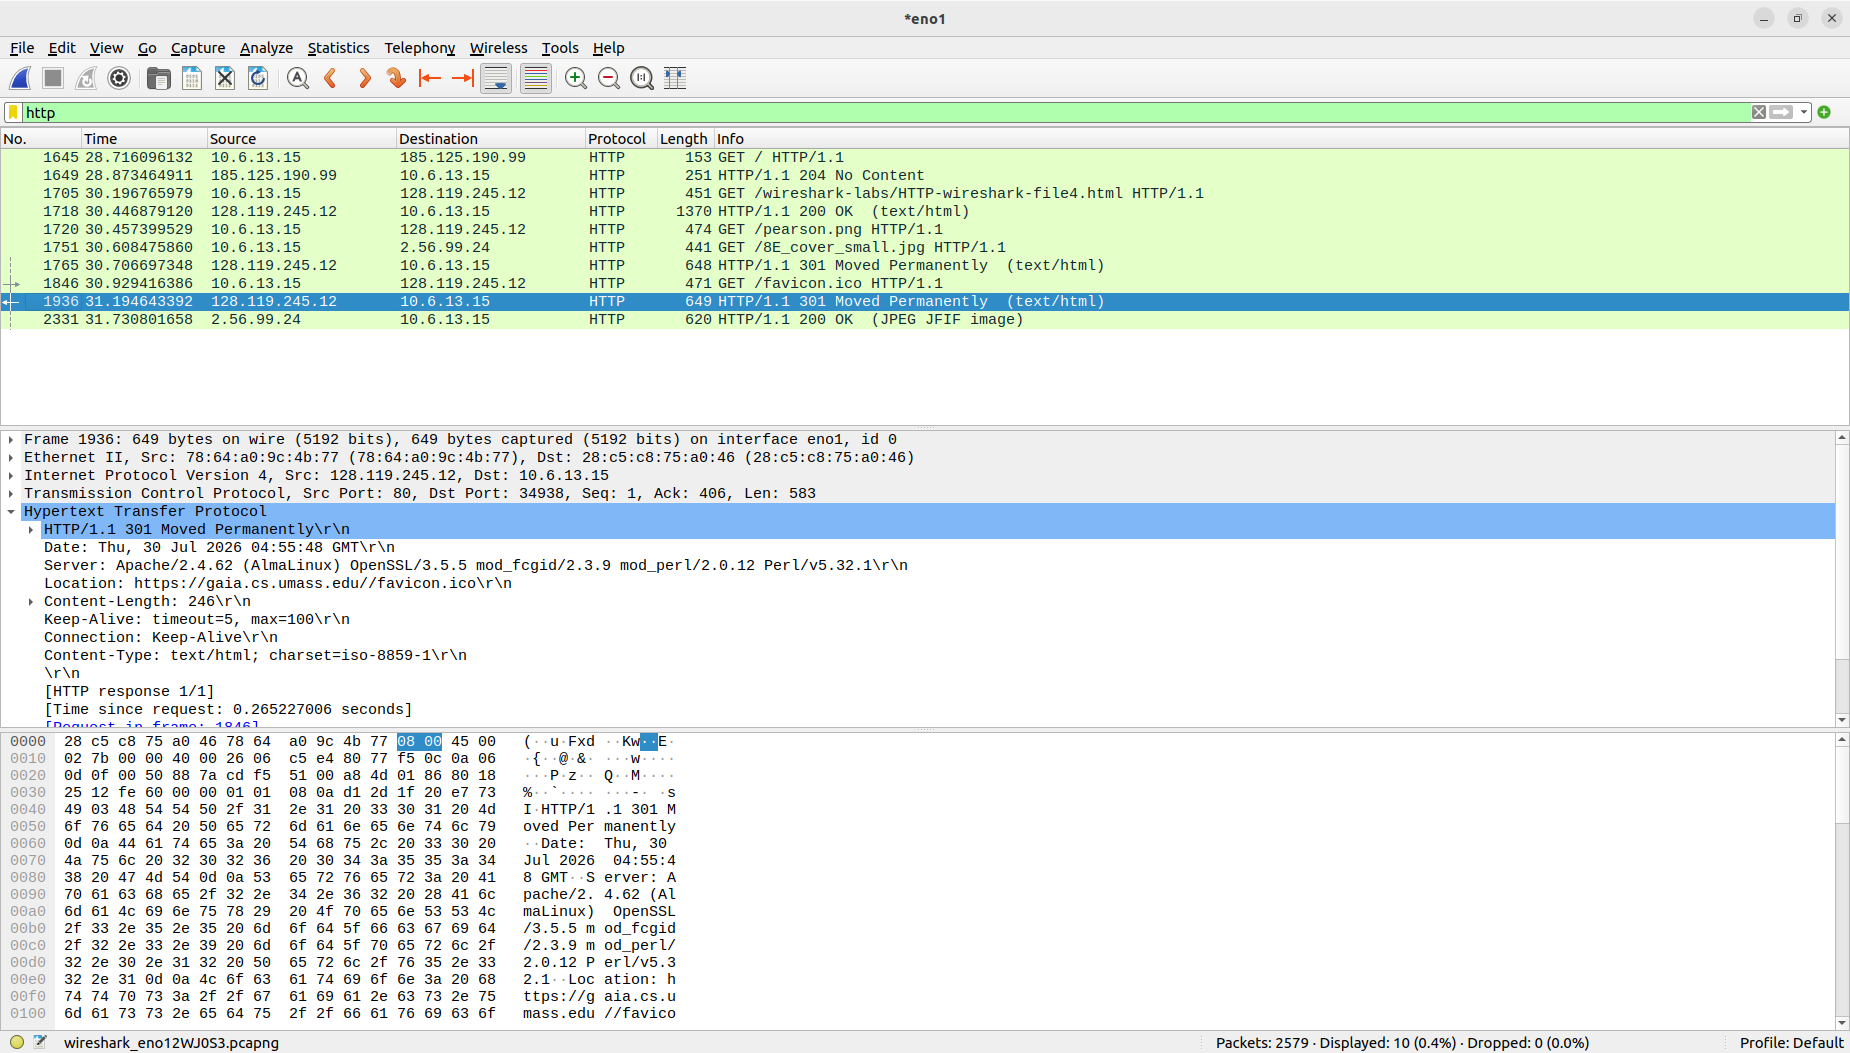
\includegraphics[width=0.95\linewidth]{shot5_embedded_objects_zoom.png}
\caption{Detail view of one of the embedded-object responses, showing response headers and raw
bytes on the wire.}
\end{figure}

\subsection*{Observations}
\begin{enumerate}
  \setcounter{enumi}{15}
  \item \textbf{GET requests sent:} Three HTTP GET requests are visible for this page load: one
        for the base HTML file (\texttt{HTTP-wireshark-file4.html}, to \texttt{128.119.245.12}),
        one for \texttt{/pearson.png} (also to \texttt{128.119.245.12}), and one for
        \texttt{/8E\_cover\_small.jpg} sent to a \emph{different} address,
        \texttt{2.56.99.24} -- confirming the lab's premise that the two embedded images are
        served from two distinct web servers.
  \item \textbf{Serial vs.\ parallel download:} The two image GET requests are issued only
        $\approx$0.15\,s apart (\texttt{30.457399529}\,s and \texttt{30.608475860}\,s) and their
        responses arrive independently at \texttt{31.194643392}\,s and \texttt{31.730801158}\,s --
        the second request is sent well before the first response is received, so the browser is
        downloading the two images \emph{in parallel} over separate TCP connections rather than
        waiting for one to finish before starting the other.
\end{enumerate}

\section*{6. Learning Outcomes}
\begin{itemize}
  \item Learned to install, configure (non-root packet capture via the \texttt{wireshark} group)
        and operate Wireshark with a display filter to isolate HTTP traffic from the rest of the
        capture.
  \item Understood the structure of an HTTP request line and header block at the byte level, and
        how to correlate the packet-list summary with the packet-detail and hex/ASCII panes.
  \item Observed that a single "page load" from a user's perspective can correspond to several
        underlying HTTP request/response exchanges (redirects, embedded objects on other hosts).
  \item Learned to distinguish serial from parallel object retrieval by comparing request and
        response timestamps across multiple TCP streams in the same capture.
  \item Reinforced how response headers (\texttt{Server}, \texttt{Location}, \texttt{Content-Length},
        \texttt{Connection}) convey server identity, redirection targets, and connection-reuse
        policy to the client.
\end{itemize}

\end{document}
